\clearpage
\section{Help Desk structure}\label{structure}
Understanding and optimizing the help desk organizational structure is an important critical success factor in achieving team and company goals.

\subsection{Structure}
Giglium will adapt the simple structure of Mintzberg\cite{mintzberg_book} to define the internal structure of the Help desk. This structure will rotate around the figure of the help desk coordinator, thanks to this fact, in the working group there is a flexible division of labor and activities. This structure is formed by the strategic apex (the help desk coordinator), which is its most important component, and by the operative core (the help desk operators), whose number will be defined in the subsections below.

\begin{figure}[h!]
	\centering
	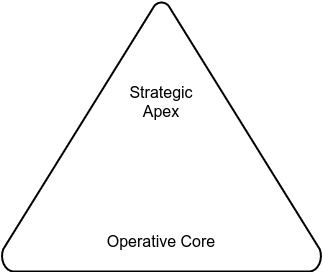
\includegraphics[width=90mm]{./img/structures/piramid.png}
	\caption{The simple structure of Mintzberg}\label{fig:piramid}
\end{figure}

The work is directly controlled by the help desk coordinator, in which there is a strong centralization of the decision-making power. This centralization allows quick decisions through an informal decision-making process. The internal relations of the working group are not institutionalized and most of the exchange information takes place between the strategic apex and the operational core. Each role represents a functional unit where it has its own functions to perform. This structure adapts easily to a simple and dynamic environment. In fact, few people would have difficulty in acting in a complex and bureaucratic environment, and, on the other hand, is a good approach to a dynamic environment. In any case, if there is no strategic apex on duty, a replacement will be temporarily appointed from the operative core.

\subsection{Kind}
\textit{\gls{perc}} has stated that it wants to release the e-lerning program on a state-by-state basis over several months. For this reason, Giglium predicts that out of the estimated two hundred and fifty copies per state sold in the first month of release, an initial service desk worker ratio of $4:250$ equal to coverage of 1.6\%. Giglium will illustrate the possible kind to suit the \textit{\gls{perc}} needs.

\subsubsection{Kind 12{-}5}\label{12_5}
To build a help desk that offers twelve hours of service (9:00 \textit{\gls{am}} to 9:00 \textit{\gls{pm}} \textit{\gls{etz}}) five days a week, Giglium recommends the following staff:
\begin{itemize}
	\item a total of two help desk coordinators;
	\item a total of six help desk operators.
\end{itemize}

\noindent Staff shifts will take place according to the table~\ref{tab:shifts_12_5}.

\paragraph{Table~\ref{tab:shifts_12_5} legend:}
\begin{itemize}
	\item Morning (\textbf{M}): from 9:00 \textit{\gls{am}} to 03:00 \textit{\gls{pm}} \textit{\gls{etz}};
	\item Afternoon (\textbf{A}): from 03:00 \textit{\gls{pm}} to 09:00 \textit{\gls{pm}} \textit{\gls{etz}};
	\item Rest (\textbf{R}): day of rest;
	\item Operator (\texttt{OP}): the help desk operator plus an identification number;
	\item Coordinator (\texttt{C}): the help desk coordinator plus an identification number.
\end{itemize}

\begin{table}[H]
	\centering
	\begin{tabular}{|l|c|c|c|c|c|c|c|c|} 
		\hline
		& \textbf{Day 1} & \textbf{Day 2} & \textbf{Day 3} & \textbf{Day 4} & \textbf{Day 5} & \textbf{Day 6} & \textbf{Day 7} & \textbf{Hours per week}\\ 
		\hline
		\texttt{C1} & M & A & M & A & A & R & R & 30\\
		\hline
		\texttt{C2} & A & M & A & M & M & R & R & 30\\
		\hline
		\texttt{OP1} & M & M & M & M & M & R & R & 30\\
		\hline
		\texttt{OP2} & A & A & A & A & A & R & R & 30\\
		\hline
		\texttt{OP3} & M & M & M & M & M & R & R & 30\\
		\hline
		\texttt{OP4} & A & A & A & A & A & R & R & 30\\
		\hline
		\texttt{OP5} & M & M & M & M & M & R & R & 30\\
		\hline
		\texttt{OP6} & A & A & A & A & A & R & R & 30\\
		\hline
	\end{tabular}
	\caption{Help desk kind 12{-}5 shifts matrix}\label{tab:shifts_12_5}
\end{table}

\subsubsection{Kind 12{-}7}\label{12_7}
To build a help desk that offers twelve hours of service (9:00 \textit{\gls{am}} to 9:00 \textit{\gls{pm}} \textit{\gls{etz}}) seven days a week, Giglium recommends the following staff:
\begin{itemize}
	\item a total of three help desk coordinators;
	\item a total of eight help desk operators.
\end{itemize}

\noindent Staff shifts will take place according to the table~\ref{tab:shifts_12_7}.

\paragraph{Table~\ref{tab:shifts_12_7} legend:}
\begin{itemize}
	\item Morning (\textbf{M}): from 09:00 \textit{\gls{am}} to 03:00 \textit{\gls{pm}} \textit{\gls{etz}};
	\item Afternoon (\textbf{A}): from 03:00 \textit{\gls{pm}} to 09:00 \textit{\gls{pm}} \textit{\gls{etz}};
	\item Rest (\textbf{R}): day of rest;
	\item Operator (\texttt{OP}): the help desk operator plus an identification number;
	\item Coordinator (\texttt{C}): the help desk coordinator plus an identification number.
\end{itemize}

\begin{table}[H]
	\centering
	\begin{tabular}{|l|c|c|c|c|c|c|c|c|} 
		\hline
		& \textbf{Day 1} & \textbf{Day 2} & \textbf{Day 3} & \textbf{Day 4} & \textbf{Day 5} & \textbf{Day 6} & \textbf{Day 7} & \textbf{Hours per week}\\ 
		\hline
		\texttt{C1} & A & M & A & M & A & R & R & 30\\
		\hline
		\texttt{C2} & M & A & M & R & R & M & A & 30\\
		\hline
		\texttt{C3} & A & R & R & A & M & A & M & 30\\
		\hline
		\texttt{OP1} & M & A & M & A & M & R & M & 36\\
		\hline
		\texttt{OP2} & A & M & A & M & R & R & A & 30\\
		\hline
		\texttt{OP3} & M & A & M & R & R & A & M & 30\\
		\hline
		\texttt{OP4} & A & M & R & R & A & M & A & 30\\
		\hline
		\texttt{OP5} & M & R & R & A & M & A & M & 30\\
		\hline
		\texttt{OP6} & R & R & A & M & A & M & A & 30\\
		\hline
		\texttt{OP7} & R & M & M & A & M & A & R & 30\\
		\hline
		\texttt{OP8} & R & A & A & M & A & M & R & 30\\
		\hline
	\end{tabular}
	\caption{Help desk kind 12{-}7 shifts matrix}\label{tab:shifts_12_7}
\end{table}

\subsubsection{Kind 24{-}5}\label{24_5}
To build a help desk that offers twenty-four hours of service (0:00 \textit{\gls{am}} to 0:00 \textit{\gls{am}} \textit{\gls{etz}}) five days a week, Giglium recommends the following staff:
\begin{itemize}
	\item a total of three help desk coordinators;
	\item a total of eight help desk operators.
\end{itemize}

\noindent Staff shifts will take place according to the table~\ref{tab:shifts_24_5}.

\paragraph{Table~\ref{tab:shifts_24_5} legend:}
\begin{itemize}
	\item Morning (\textbf{M}): from 07:00 \textit{\gls{am}} to 03:00 \textit{\gls{pm}} \textit{\gls{etz}};
	\item Afternoon (\textbf{A}): from 03:00 \textit{\gls{pm}} to 11:00 \textit{\gls{pm}} \textit{\gls{etz}};
	\item Night (\textbf{N}): from 11:00 \textit{\gls{pm}} to 07:00 \textit{\gls{am}} \textit{\gls{etz}};
	\item Rest (\textbf{R}): day of rest;
	\item Operator (\texttt{OP}): the help desk operator plus an identification number;
	\item Coordinator (\texttt{C}): the help desk coordinator plus an identification number.
\end{itemize}

\begin{table}[H]
	\centering
	\begin{tabular}{|l|c|c|c|c|c|c|c|c|} 
		\hline
		& \textbf{Day 1} & \textbf{Day 2} & \textbf{Day 3} & \textbf{Day 4} & \textbf{Day 5} & \textbf{Day 6} & \textbf{Day 7} & \textbf{Hours per week}\\ 
		\hline
		\texttt{C1} & M & A & M & A & A & R & R & 40\\
		\hline
		\texttt{C2} & A & M & A & M & M & R & R & 40\\
		\hline
		\texttt{C2} & N & N & N & N & N & R & R & 40\\
		\hline
		\texttt{OP1} & M & M & M & M & M & R & R & 40\\
		\hline
		\texttt{OP2} & A & A & A & A & A & R & R & 40\\
		\hline
		\texttt{OP3} & M & M & M & M & M & R & R & 40\\
		\hline
		\texttt{OP4} & A & A & A & A & A & R & R & 40\\
		\hline
		\texttt{OP5} & M & M & M & M & M & R & R & 40\\
		\hline
		\texttt{OP6} & A & A & A & A & A & R & R & 40\\
		\hline
		\texttt{OP7} & N & N & N & N & N & R & R & 40\\
		\hline
		\texttt{OP8} & N & N & N & N & N & R & R & 40\\
		\hline
	\end{tabular}
	\caption{Help desk kind 24{-}5 shifts matrix}\label{tab:shifts_24_5}
\end{table}

\begin{tcolorbox}
	During the night shift, Giglium expects far fewer users than the other shifts for this the initial service desk worker ratio will be reduced to $3:250$ equal to coverage of 1.2\%.
\end{tcolorbox}

\subsubsection{Kind 24{-}7}\label{24_7}
To build a help desk that offers twenty-four hours of service (0:00 \textit{\gls{am}} to 0:00 \textit{\gls{am}} \textit{\gls{etz}}) seven days a week, Giglium recommends the following staff:
\begin{itemize}
	\item a total of five help desk coordinators;
	\item a total of ten help desk operators.
\end{itemize}

\noindent Staff shifts will take place according to the table~\ref{tab:shifts_24_7}.

\paragraph{Table~\ref{tab:shifts_24_7} legend:}
\begin{itemize}
	\item Morning (\textbf{M}): from 07:00 \textit{\gls{am}} to 03:00 \textit{\gls{pm}} \textit{\gls{etz}};
	\item Afternoon (\textbf{A}): from 03:00 \textit{\gls{pm}} to 11:00 \textit{\gls{pm}} \textit{\gls{etz}};
	\item Night (\textbf{N}): from 11:00 \textit{\gls{pm}} to 07:00 \textit{\gls{am}} \textit{\gls{etz}};
	\item Rest (\textbf{R}): day of rest;
	\item Operator (\texttt{OP}): the help desk operator plus an identification number;
	\item Coordinator (\texttt{C}): the help desk coordinator plus an identification number.
\end{itemize}

\begin{table}[H]
	\centering
	\begin{tabular}{|l|c|c|c|c|c|c|c|c|} 
		\hline
		& \textbf{Day 1} & \textbf{Day 2} & \textbf{Day 3} & \textbf{Day 4} & \textbf{Day 5} & \textbf{Day 6} & \textbf{Day 7} & \textbf{Hours per week}\\ 
		\hline
		\texttt{C1} & A & M & A & M & A & R & R & 40\\
		\hline
		\texttt{C2} & M & A & M & R & R & M & A & 40\\
		\hline
		\texttt{C3} & A & R & R & A & M & A & M & 40\\
		\hline
		\texttt{C4} & N & N & N & N & R & R & N & 40\\
		\hline
		\texttt{C5} & N & N & R & R & N & N & N & 40\\
		\hline
		\texttt{OP1} & M & A & M & A & M & R & R & 40\\
		\hline
		\texttt{OP2} & A & M & A & M & R & R & A & 40\\
		\hline
		\texttt{OP3} & M & A & M & R & R & A & M & 40\\
		\hline
		\texttt{OP4} & A & M & R & R & A & M & A & 40\\
		\hline
		\texttt{OP5} & M & R & R & A & M & A & M & 40\\
		\hline
		\texttt{OP6} & R & R & A & M & A & M & A & 40\\
		\hline
		\texttt{OP7} & R & M & M & A & M & A & R & 40\\
		\hline
		\texttt{OP8} & R & A & A & M & A & M & R & 40\\
		\hline
		\texttt{OP9} & N & R & N & N & N & N & R & 40\\
		\hline
		\texttt{OP10} & R & N & N & N & N & R & M & 40\\
		\hline
	\end{tabular}
	\caption{Help desk kind 12{-}7 shifts matrix}\label{tab:shifts_24_7}
\end{table}

\begin{tcolorbox}
	During the night shift, Giglium expects far fewer users than the other shifts for this, the initial service desk worker ratio will be reduced to $3:250$ equal to coverage of 1.2\%. 
	
	During the night shift on weekends, Giglium expects even fewer users than the night shift and for this the initial service desk employment ratio will be reduced to $2:250$ equal to coverage of 0.8\%.
\end{tcolorbox}

\subsection{Management of working hours and shifts}
The help desk coordinators are responsible for scheduling the shifts which must comply with the contractual obligation hours and be consistent with the established service hours. The same are required to draw up and present the monthly hourly prospectuses of the operators distributed on several shifts, by the 25th of the previous month. These shifts may vary according to the availability of staff (holidays, daily leave, and sickness) and it will be the responsibility of the help desk coordinator to promptly notify \textit{\gls{perc}} of any changes.

The main criteria for scheduling working hours and shifts are described in the following bullet:
\begin{itemize}
	\item in the case of kind 12{-}5 (see: section~\ref{12_5}) or 12{-}7 (see: section~\ref{12_7}) the average duration of the working hours cannot exceed 40 hours every seven days (including extraordinary), since all the help desk coordinator and operators have a part-time contract;
	\item in the case of kind 24{-}5 (see: section~\ref{24_5}) or 24{-}7 (see: section~\ref{24_7}) the average duration of the working hours cannot exceed 48 hours every seven days (including extraordinary), since all the help desk coordinator and operators have a full-time contract;
	\item if the daily working hours exceed 6 hours, the worker has the right to a lasting break
	not less than 10 minutes;
	\item Each worker must benefit, over a period of 24 hours, in no less than 11 consecutive hours of daily rest;
	\item the night period is a period of at least seven consecutive hours including the interval between midnight and five in the morning (from 00:00 \textit{\gls{am}} at 5:00 \textit{\gls{pm}} \textit{\gls{etz}}). Specific suitability for night work is ascertained through the Competent Doctor. A worker without the doctor approval cannot perform any night shifts;
	\item a help desk coordinator need to be always available. In any case, if there is no help desk coordinator on duty, a replacement will be temporarily appointed from the operators;
	\item the initial service desk ratio are indicative and not binding to be manteing to be manteing.
\end{itemize}